\section{Before scaling: discriminating mechanisms from interface burden}
\label{sec:prescale}
The next stage is not simply more seeds. We first separate three tractable
questions: whether a proposer can submit its intended design, whether an
institution has an actual native consumer, and whether objective-conditioned
revision changes native outcomes. Only the last is new optimization evidence.
The following additions have distinct statuses; they are not folded into the
closed V2 benchmark or its unchanged selection.

\subsection{What the closed record already explains}
A read-only analysis of all 120 V2 statuses retains 64 measured profiles and
nine reference profiles reconstructed from their three affine loss scores.
Those nine reconstructions are not new raw measurements. In the observed
coefficient family $L_{\alpha,\beta}=\alpha A-Q+\beta R$, the original
$C$ coefficients $(4,0.1)$ favor reviewer-free rejection over the observed
high-$Q$ profile. This follows from proxy geometry, not necessarily a weak
optimizer. The map is only over observed profiles; it is not a bound or optimum
for untried dynamic policies (Figure~\ref{fig:observed-objective-map}).

\begin{figure}[t]
\centering
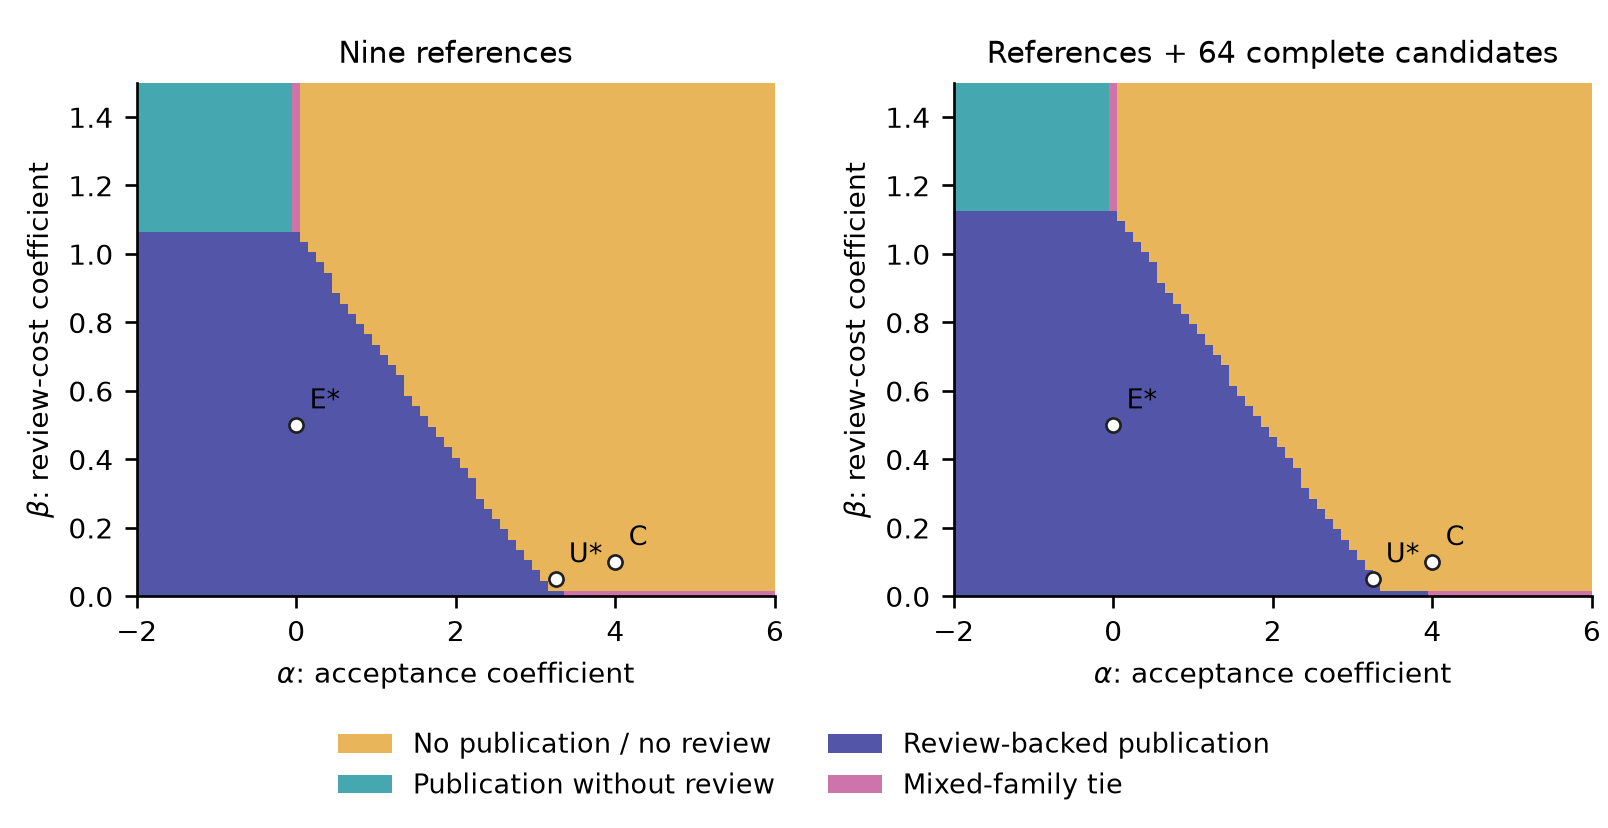
\includegraphics[width=\linewidth]{figures/pre-scale/observed-objective-map-print.png}
\caption{Post-hoc objective geometry over observed development profiles,
not new objective-conditioned search. Left: nine reference-score inversions;
right: those references plus 64 measured completed candidates. Colors identify
observed outcome families, not general policy equivalence. The coefficient
grid is a plotting choice, not additional samples or global optimality.
C is the original V2 loss; E*/U* mark diagnostic formulas, not new searches.}
\label{fig:observed-objective-map}
\end{figure}

Likewise, the numeric failures are not an absence of submission attempts.
Their 384 editor steps contain 47 finish rejections: 43 outside the declared
numeric-only domain and four out-of-range. Of 228 reads, 166 target existing
selection source. This describes a presentation/compliance confound and does
not identify a single proven cognitive or transport cause. A new interface
must be tested prospectively rather than repairing these failed slots.

\subsection{Literal numerical submission: a limited real-backend result}
The new numerical interface asks for exactly six typed coordinate values and
an uninterpreted rationale. Values compile literally to a patch under the same
declared domain; there is no clipping, code repair or implicit baseline. A
complete explicit parent assignment is valid retention. Finite semantic-call
and whole-session wall budgets, durable exact wire bytes, raw responses and
cold replay distinguish known invalid replies from unknown completion.

At pinned source~\code{215311c}, two predeclared local 35B readiness cases both
complete on their first generation call (Table~\ref{tab:numeric-readiness}).
No native world is evaluated. In particular, the E rationale incorrectly
conjectures that limiting delivered history records could directly reduce the
review-count metric; preserving a valid literal submission does not validate
that explanation. The result establishes interface execution for these two
requests, not an optimized loss, general editor readiness or designer competence.
Later runtime changes require a new source-specific certificate.

\begin{table}[t]
\centering\small
\begin{tabular}{@{}lrrll@{}}
\toprule
Case & Prompt tokens & Output tokens & Literal action & Native loss\\
\midrule
T &3196&285&Explicit parent retention&Not observed\\
E &3340&993&Different valid coordinates&Not observed\\
\bottomrule
\end{tabular}
\caption{Actual local 35B numerical readiness, two generation POSTs. Recorded
HTTP call times are 6.972 and 14.056 seconds, excluding separate role loading and
other overhead. Both submissions cold-replay. This is not a search comparison.}
\label{tab:numeric-readiness}
\end{table}

\subsection{A native information-path intervention, not another toy world}
A developer-authored history office now reads actual native papers, statuses
and review summaries, with bounded records per researcher. M0 runs the
producer without delivery; M1 delivers own history; M2 delivers society
history; M3 delays own history an additional year. All retain the original
scientific activities and remove the old example's direct project reassignment.
M2 is not an exactly token-matched inert placebo. Original-world tests with
scripted HTTP/corpus and real isolated code execution verify first direction
input years absent/2/2/3 and full pre-delivery payload equality under different
host clocks. These are software/effect-path tests, not fresh Qwen outcomes.

The finite actual study declares three development seeds and four years,
at most 12 worlds. At the recorded observation on November 9, the first world
has started, initial direction replies exist, and the missing four-year
literature embedding index is being built on CPU. No terminal world
observation is available. This status does not imply completed scientific
results or a continuing live heartbeat in the manuscript.

A separate prospective source implements T/E search over numerical, fixed-graph
code, code/graph and uniform proposals: two generations, at most 16 candidate
worlds plus six fresh references. The selected policies are frozen before at
most 36 four-year unused-seed evaluations. The pilot explicitly fixes original
production/calendar/accounting effects, while permitting institutional
algorithms, entities, memory and routes to change. This is a declared design
domain, not an additional outcome veto or the global expressive ceiling.
Source-specific numerical and staged-editor readiness gates precede dispatch.
At this manuscript revision, this search/evaluation is implemented but not
executed; it supplies no additional optimizer outcome.

\subsection{Verifiable activities and continuity at the same boundary}
An opt-in claim-verification consumer checks an institution's literal assertion
about counts of actual native accept/reject decisions or review records over
a completed interval. It reads the simulator's archive independently of the
candidate's observation or proposed verdict. A correction has a new identity,
retains the false predecessor and binds its verification hash. Retained state
is checked against actual evidence, rather than accepting a designer-seeded
\code{matches=true} flag. Scientific text remains literal; a source-owned
operational review-time field is excluded only from the count-evidence identity.

Original-world/Docker software tests connect authored false assertion,
independent verification, correction and actual next-year researcher input.
This is internally checkable empirical work about the simulated society,
\emph{not} verification of the truth of retrieved scientific papers or a new
scientific-value objective. No default phase or hidden merit gate is added.

Additional scripted native tests place the existing antithetic score estimator
on the current information institution, execute its updated parameter in a
fresh native forward and retain a no-gradient control. A same-society test
changes the history mechanism while preserving researchers, papers, resources,
mechanism memory, RNG state and pending delayed deliveries. These establish
current-boundary connectivity, not new live-model gradients, practical method
advantage, autonomous invention or recursive improvement. The English
pre-scale observatory presents only timestamped journal observations, explicitly
distinguishing a start without a terminal record from a verified completion.
